\section{Study the dataset}

The two datasets chosen from the UCI Machine Learning repository are:
\href{https://archive.ics.uci.edu/dataset/186/wine+quality}{Wine Quality}
and \href{https://archive.ics.uci.edu/dataset/19/car+evaluation}{Car Evaluation}.

\subsection{Wine Quality}

"Two datasets are included, related to red and white vinho verde wine samples,
from the north of Portugal. The goal is to model wine quality based on
physicochemical tests."

\subsubsection{Features classification}

All but two features in the Wine Quality dataset are continuous and
quantitative, because they represent measureable values that can
take on an infinite number of values within a certain range.
Continuous data can be represented by fractions, decimals or whole
numbers. Quantitative data deals with numerical information that
can be measured or counted.

In the Wine Quality dataset, most of its features - fixed acidity,
volatile acidity, citric acid, residual sugar, etc. represents
the physiochemical properties of vinho verde wine. They can be any
value between a certain range, so they are continuous and
quantitative.

The remaining two features, quality and color are discrete. Quality
is also quantitative, since it's represented by an integer between
0 and 10. Color is qualitative, since it categorizes the sample by
its color, either "red" or "white".

\subsubsection{Statistics}

\begin{table}[!h]
    \begin{center}
        \begin{tabular}{lrr}
            \toprule
            {} &           mean & variance \\
            \midrule
            fixed\_acidity         &    7.215307  &     1.680740 \\
            volatile\_acidity      &    0.339666  &     0.027105 \\
            citric\_acid           &    0.318633  &     0.021117 \\
            residual\_sugar        &    5.443235  &    22.636696 \\
            chlorides              &    0.056034  &     0.001227 \\
            free\_sulfur\_dioxide  &   30.525319  &   315.041192 \\
            total\_sulfur\_dioxide &  115.744574  &  3194.720039 \\
            density                &    0.994697  &     0.000009 \\
            pH                     &    3.218501  &     0.025853 \\
            sulphates              &    0.531268  &     0.022143 \\
            alcohol                &   10.491801  &     1.422561 \\
            \bottomrule
        \end{tabular}
        \caption{Mean and variance of the Wine Quality dataset}
    \end{center}
\end{table}

\begin{table}[!h]
    \begin{center}
    \resizebox{\textwidth}{!}{
        \begin{tabular}{lrrrrrrrrrrr}
            \toprule
            {} &  fixed\_acidity &  volatile\_acidity &  citric\_acid &  residual\_sugar &  chlorides &  free\_sulfur\_dioxide &  total\_sulfur\_dioxide &   density &        pH &  sulphates &    alcohol \\
            \midrule
            fixed\_acidity        &       1.680740 &          0.046745 &     0.061122 &       -0.690720 &   0.013544 &            -6.506003 &            -24.112030 &  0.001784 & -0.052675 &   0.057792 &  -0.147594 \\
            volatile\_acidity     &       0.046745 &          0.027105 &    -0.009043 &       -0.153537 &   0.002175 &            -1.030242 &             -3.856933 &  0.000134 &  0.006921 &   0.005536 &  -0.007391 \\
            citric\_acid          &       0.061122 &         -0.009043 &     0.021117 &        0.098490 &   0.000199 &             0.343372 &              1.603646 &  0.000042 & -0.007706 &   0.001215 &  -0.001819 \\
            residual\_sugar       &      -0.690720 &         -0.153537 &     0.098490 &       22.636696 &  -0.021492 &            34.021685 &            133.244854 &  0.007883 & -0.204498 &  -0.131635 &  -2.039567 \\
            chlorides            &       0.013544 &          0.002175 &     0.000199 &       -0.021492 &   0.001227 &            -0.121284 &             -0.553714 &  0.000038 &  0.000252 &   0.002062 &  -0.010735 \\
            free\_sulfur\_dioxide  &      -6.506003 &         -1.030242 &     0.343372 &       34.021685 &  -0.121284 &           315.041192 &            723.261972 &  0.001369 & -0.416249 &  -0.497756 &  -3.807165 \\
            total\_sulfur\_dioxide &     -24.112030 &         -3.856933 &     1.603646 &      133.244854 &  -0.553714 &           723.261972 &           3194.720039 &  0.005491 & -2.166696 &  -2.319079 & -17.914646 \\
            density              &       0.001784 &          0.000134 &     0.000042 &        0.007883 &   0.000038 &             0.001369 &              0.005491 &  0.000009 &  0.000006 &   0.000116 &  -0.002456 \\
            pH                   &      -0.052675 &          0.006921 &    -0.007706 &       -0.204498 &   0.000252 &            -0.416249 &             -2.166696 &  0.000006 &  0.025853 &   0.004597 &   0.023252 \\
            sulphates            &       0.057792 &          0.005536 &     0.001215 &       -0.131635 &   0.002062 &            -0.497756 &             -2.319079 &  0.000116 &  0.004597 &   0.022143 &  -0.000538 \\
            alcohol              &      -0.147594 &         -0.007391 &    -0.001819 &       -2.039567 &  -0.010735 &            -3.807165 &            -17.914646 & -0.002456 &  0.023252 &  -0.000538 &   1.422561 \\
            \bottomrule
        \end{tabular}
    }
    \caption{Covariance of the Wine Quality dataset}
    \end{center}
\end{table}

\begin{table}[!h]
    \begin{center}
    \resizebox{\textwidth}{!}{
        \begin{tabular}{lrrrrrrrrrrr}
            \toprule
            {} &  fixed\_acidity &  volatile\_acidity &  citric\_acid &  residual\_sugar &  chlorides &  free\_sulfur\_dioxide &  total\_sulfur\_dioxide &   density &        pH &  sulphates &   alcohol \\
            \midrule
            fixed\_acidity        &       1.000000 &          0.219008 &     0.324436 &       -0.111981 &   0.298195 &            -0.282735 &             -0.329054 &  0.458910 & -0.252700 &   0.299568 & -0.095452 \\
            volatile\_acidity     &       0.219008 &          1.000000 &    -0.377981 &       -0.196011 &   0.377124 &            -0.352557 &             -0.414476 &  0.271296 &  0.261454 &   0.225984 & -0.037640 \\
            citric\_acid          &       0.324436 &         -0.377981 &     1.000000 &        0.142451 &   0.038998 &             0.133126 &              0.195242 &  0.096154 & -0.329808 &   0.056197 & -0.010493 \\
            residual\_sugar       &      -0.111981 &         -0.196011 &     0.142451 &        1.000000 &  -0.128940 &             0.402871 &              0.495482 &  0.552517 & -0.267320 &  -0.185927 & -0.359415 \\
            chlorides            &       0.298195 &          0.377124 &     0.038998 &       -0.128940 &   1.000000 &            -0.195045 &             -0.279630 &  0.362615 &  0.044708 &   0.395593 & -0.256916 \\
            free\_sulfur\_dioxide  &      -0.282735 &         -0.352557 &     0.133126 &        0.402871 &  -0.195045 &             1.000000 &              0.720934 &  0.025717 & -0.145854 &  -0.188457 & -0.179838 \\
            total\_sulfur\_dioxide &      -0.329054 &         -0.414476 &     0.195242 &        0.495482 &  -0.279630 &             0.720934 &              1.000000 &  0.032395 & -0.238413 &  -0.275727 & -0.265740 \\
            density              &       0.458910 &          0.271296 &     0.096154 &        0.552517 &   0.362615 &             0.025717 &              0.032395 &  1.000000 &  0.011686 &   0.259478 & -0.686745 \\
            pH                   &      -0.252700 &          0.261454 &    -0.329808 &       -0.267320 &   0.044708 &            -0.145854 &             -0.238413 &  0.011686 &  1.000000 &   0.192123 &  0.121248 \\
            sulphates            &       0.299568 &          0.225984 &     0.056197 &       -0.185927 &   0.395593 &            -0.188457 &             -0.275727 &  0.259478 &  0.192123 &   1.000000 & -0.003029 \\
            alcohol              &      -0.095452 &         -0.037640 &    -0.010493 &       -0.359415 &  -0.256916 &            -0.179838 &             -0.265740 & -0.686745 &  0.121248 &  -0.003029 &  1.000000 \\
            \bottomrule
        \end{tabular}
    }
    \caption{Correlation of the Wine Quality dataset}
    \end{center}
\end{table}

\newpage

\subsubsection{Comments on the correlation of features in the dataset}

\begin{itemize}
    \item Free sulfur dioxide and total sulfur dioxide are highly correlated (0.720934).
    \item Density and residual sugar are highly correlated (0.552517).
    \item Density and alcohol are highly negatively correlated (-0.686745).
    \item Total sulfur dioxide and volatile acidity are negatively correlated (-0.414476).
\end{itemize}

\subsection{Car Evaluation}

Derived from simple hierarchical decision model, this database may be useful
for testing constructive induction and structure discovery methods. 

\subsubsection{Features classification}

All features are categorical and qualitative, as they represent distinct
categories, cannot be ordered and they deal with descriptive information instead
of numerical values.

\begin{itemize}
    \item \textbf{buying:} relative cost of buying the car.
    \item \textbf{maint:} relative maintenance cost of the car.
    \item \textbf{doors:} number of doors in the car.
    \item \textbf{persons:} passenger capacity of the car.
    \item \textbf{lug\_boot:} size of the luggage boot.
    \item \textbf{safety:} estimated safety level of the car.
\end{itemize}

\subsubsection{Statistics}

\begin{table}[!h]
    \begin{center}
        \begin{tabular}{lrr}
            \toprule
            {} &    mean & variance \\
            \midrule
            buying   &  1.5 &  1.250724  \\
            maint    &  1.5 &  1.250724  \\
            doors    &  1.5 &  1.250724  \\
            persons  &  1.0 &  0.667053 \\
            lug\_boot &  1.0 &  0.667053  \\
            \bottomrule
        \end{tabular}
        \caption{Mean and variance of the Car Evaluation dataset}
    \end{center}
\end{table}

\begin{table}[!h]
    \begin{center}
        \begin{tabular}{lrrrrr}
            \toprule
            {} &    buying &     maint &     doors &   persons &  lug\_boot \\
            \midrule
            buying   &  1.250724 &  0.000000 &  0.000000 &  0.000000 &  0.000000 \\
            maint    &  0.000000 &  1.250724 &  0.000000 &  0.000000 &  0.000000 \\
            doors    &  0.000000 &  0.000000 &  1.250724 &  0.000000 &  0.000000 \\
            persons  &  0.000000 &  0.000000 &  0.000000 &  0.667053 &  0.000000 \\
            lug\_boot &  0.000000 &  0.000000 &  0.000000 &  0.000000 &  0.667053 \\
            \bottomrule
        \end{tabular}
        \caption{Covariance of the Car Evaluation dataset}
    \end{center}
\end{table}

\begin{table}[!h]
    \begin{center}
        \begin{tabular}{lrrrrr}
            \toprule
            {} &        buying &         maint &         doors &       persons &      lug\_boot \\
            \midrule
            buying   &  1.000000e+00 & -3.436808e-16 & -2.097088e-16 & -4.089152e-17 & -1.691262e-16 \\
            maint    & -3.436808e-16 &  1.000000e+00 & -6.466021e-17 & -4.272143e-17 & -1.549092e-16 \\
            doors    & -2.097088e-16 & -6.466021e-17 &  1.000000e+00 &  1.956599e-17 & -1.942523e-17 \\
            persons  & -4.089152e-17 & -4.272143e-17 &  1.956599e-17 &  1.000000e+00 &  3.854941e-18 \\
            lug\_boot & -1.691262e-16 & -1.549092e-16 & -1.942523e-17 &  3.854941e-18 &  1.000000e+00 \\
            \bottomrule
        \end{tabular}
        \caption{Correlation of the Car Evaluation dataset}
    \end{center}
\end{table}

\subsubsection{Comments on the correlation of features in the dataset}

Nothing is correlated to eachother, and each criteria of the car evaluation is
independent from eachother. In other words, there are no meaningful relationship
between any two criterias.

\section{PCA - Principal Component Analysis}

\subsection{Car Evaluation}

\subsubsection{With 2 principal components}

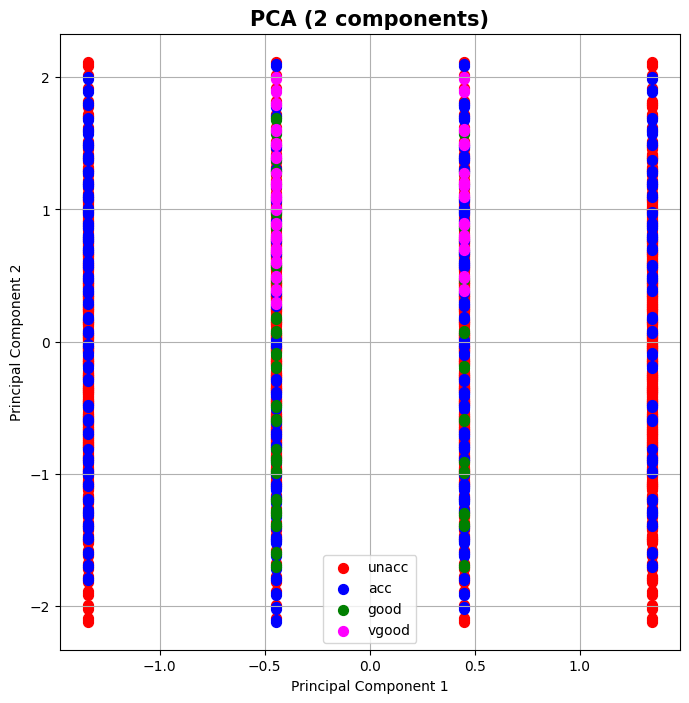
\includegraphics{car_pca_2_components.png}

The first two principal components account for 33.3\% (split equally into 16.6\%
each) of the total variation in the dataset. It can be clearly seen that there
are four distinct columns, most likely corresponding to the four possible
values of the three attributes: buying, maint and doors. Some patterns can be
observed from the graph above:

\begin{itemize}
    \item The two columns on the far left and right only contain the "unacc" and "acc" classes.
    \item The "good" and "vgood" classes only appear in the columns in the middle.
    \item The "vgood" class only appears if the second principal component has a value higher than 0.
\end{itemize}

The points in the graph heavily overlap, but in a very specific manner as shown
in the graph and the above presented points. Thus, we can conclude that the
classes are relatively well-separated and the classes are clustered distinctly
from eachother. In conclusion, the two principal components used are sufficient
for data representation, despite their low explained variance value.

\subsubsection{With 3 principal components}

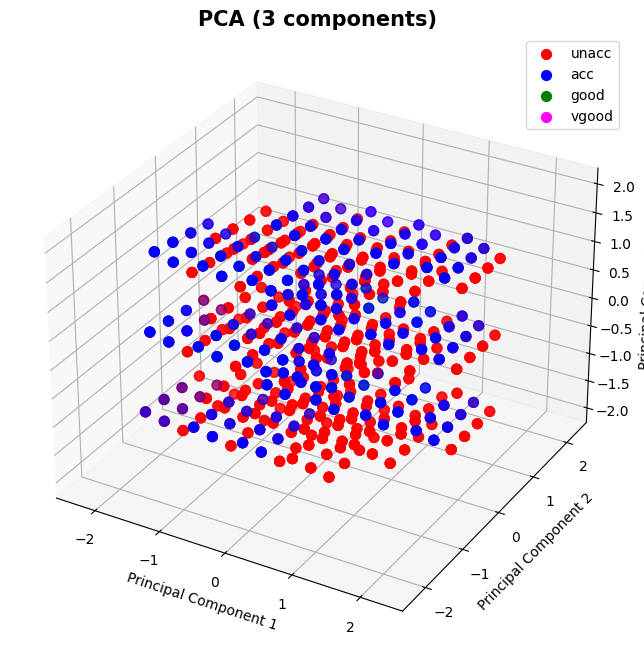
\includegraphics{car_pca_3_components.png}

Having a third principal component increases the total explained variance value
by another 16.6\%, to a 50\%, representing half of the differences between
the four classes. Despite an increase in the total explained variance, the
clarity of the visualization is negatively impacted - the data points in the
plot heavily overlap, with classes being less separated and no distinct clusters
are to be seen. In conclusion, the addition of a third principal component
does not improve the separation of classes, but worsens the representation
significantly.